% ---------------------------------------------------------------------------- %
\subsection{Systemaufbau}
\label{subsec:sysaufbau}
% ---------------------------------------------------------------------------- %

Unter  einem  Kombipendel  wollen  wir  ein  System  verstehen,  bei  dem  die
R\"uckstellungskr\"afte sowohl  von der Gravitationskraft wie  auch von Federn
generiert  werden. In diesem  Versuch  wurde eine  Apparatur in  verschiedenen
Konfigurationen  benutzt, deren  Aufbau  in Abbildung  \ref{fig:pendelKonfigs}
gesehen werden kann.

\begin{figure}[h!]
    \centering
    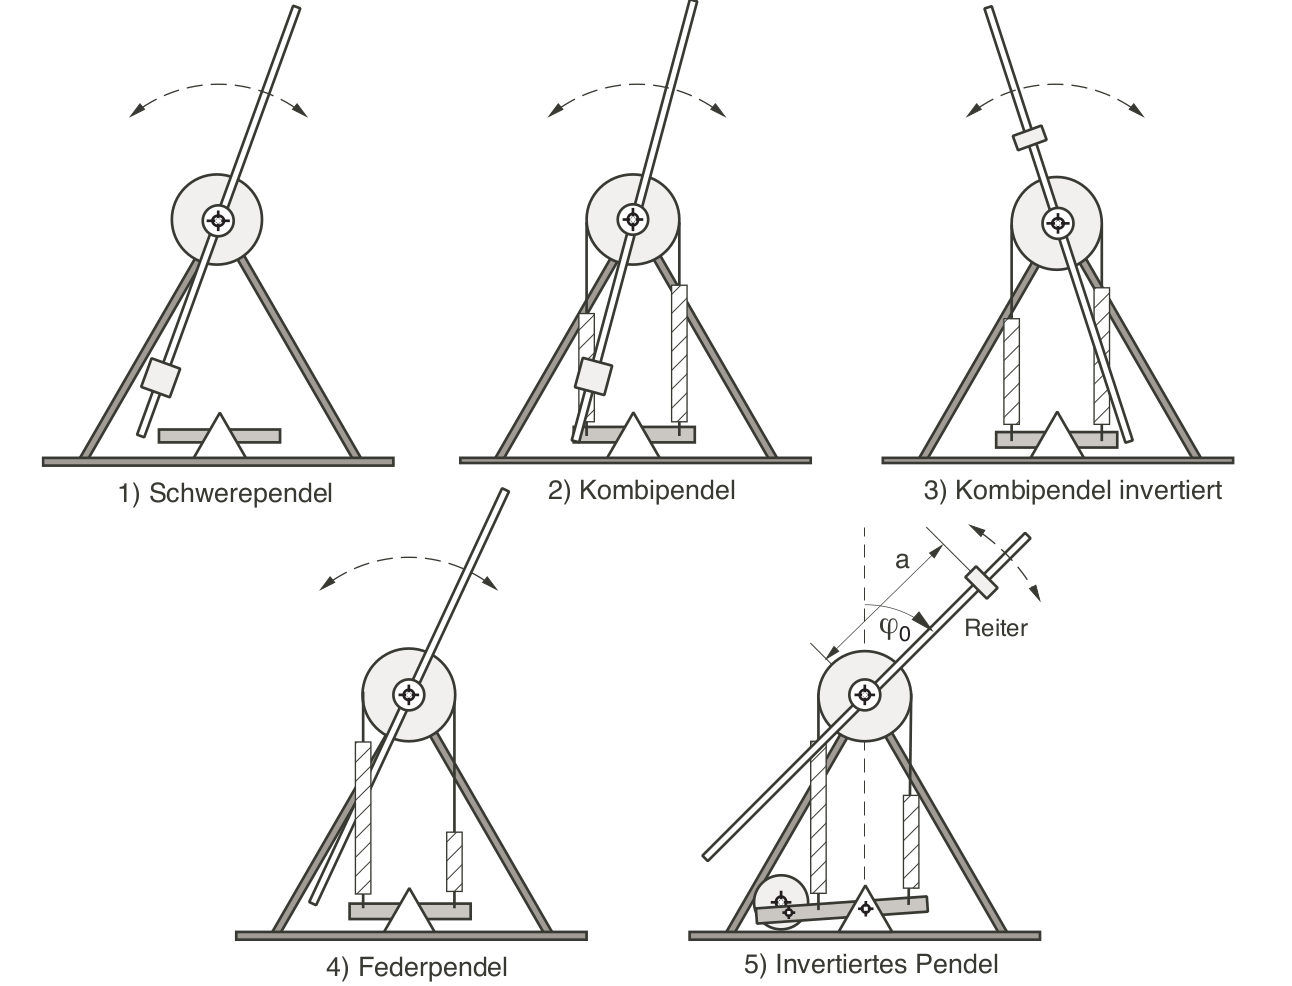
\includegraphics[width=\textwidth]{images/pendel-konfigs.png}
    \caption{%
        Pendel-Konfigurationen. Quelle: Versuchsanleitung.
    }
    \label{fig:pendelKonfigs}
\end{figure}

\begin{enumerate}
    \item
        ohne Federn als Schwerependel
    \item
        mit Ruhelage unten $\varphi_0 = \SI{180}{\degree}$ als quasiharmonisches Kombipendel
    \item
        mit Ruhelage oben $\varphi_0 = \SI{0}{\degree}$ als quasiharmonisches Kombipendel invertiert
    \item
        mit ausbalanciertem Pendelk\"orper als Federpendel (Drehpendel)
    \item
        mit Ruhelage oben ($\SI{0}{\degree} < \varphi_0 < \SI{120}{\degree}$) als invertiertes Pendel
\end{enumerate}


% ---------------------------------------------------------------------------- %
\subsection{Schwerependel}
\label{subsec:theorie:schwerependel}
% ---------------------------------------------------------------------------- %

% ---------------------------------------------------------------------------- %
\subsubsection{Reiterabstand variabel}
\label{subsec:schwerependel:reitervar}
% ---------------------------------------------------------------------------- %
F\"ur kleine Auslenkungen kann die Schwingungsperiode des Schwerependels bestimmt werden via

\begin{equation}
    T_0 = 2 \cdot \pi \cdot \sqrt{\frac{I_0 + m_{Reiter} \cdot a^2}{m_{Reiter} \cdot g \cdot a}}
\end{equation}

Wobei

\begin{itemize}
    \item
        $T_0$: Schwingungsperiode
    \item
        $I_0$: Massentr\"agheitsmoment der leeren Apparatur (ohne Reiter). Fit-Parameter.
    \item
        $m_{Reiter}$: Reitermasse
    \item
        $a$: Position des Reiters (Entfernung des Mittelpunktes des Reiters zum Mittelpunkt der Pendelstange)
    \item
        $g$: Erdbeschleunigung. Gem\"ass Angaben im Labor \SI{9.807}{\meter\per\second\squared}
\end{itemize}

Im Z\"ahler unter  der Wurzel steht eigentlich  das gesamte Tr\"agheitsmoment,
welches  durch die  Schwingung  in Bewegung  gesetzt wird. Beim  Schwerependel
ist  dies  das  Tr\"agheitsmoment  der  Apparatur  und  das  Tr\"agheitsmoment
des   Reiters  (beim   Kombipendel  kommt   noch  das   Tr\"agheitsmoment  der
Federn  hinzu). Der   Term  $m_{Reiter}  \cdot  a^2$   ist  die  Approximation
des   Tr\"agheitsmoments   des   Reiters   als   Punktmasse. Bei   gr\"osseren
Reitersn   (\SI{400}{\gram}    und   h\"oher)   sollte   dieses    durch   das
Massentr\"agheitsmoment  eines  Zylinders  mit  entsprechendem  Steiner-Anteil
ersetzt werden (siehe auch Abschnitt \ref{subsec:periodeReitermasse} auf Seite
\pageref{subsec:periodeReitermasse}).


% ---------------------------------------------------------------------------- %
\subsubsection{Auslenkung variabel}
\label{subsec:schwerependel:amplivar}
% ---------------------------------------------------------------------------- %

Variiert  man  die  Auslenkung  (also  den Winkel,  aus  dem  man  das  Pendel
losl\"asst), kann die Periode der Schwingung mit folgender Formel angen\"ahert
werden:

\begin{equation}
    T = T_0 \cdot
        \left(
            1 +
            \left( \frac{1}{2} \right)^2 \cdot sin^2 \left( \frac{\hat{\varphi}}{2} \right)
            \left( \frac{1 \cdot 3}{2 \cdot 4} \right)^2 \cdot sin^4 \left( \frac{\hat{\varphi}}{2} \right)
            \left( \frac{1 \cdot 3 \cdot 5}{2 \cdot 4 \cdot 6} \right)^2 \cdot sin^6 \left( \frac{\hat{\varphi}}{2} \right)
            + ...
        \right)
\end{equation}

Wobei gilt:
\begin{itemize}
    \item
        $T$: Schwingungsperiode
    \item
        $T_0$: Schwingungsperiode f\"ur kleine Auslenkungen
    \item
        $\hat{\varphi}$: Amplitude der Schwingung
\end{itemize}

Die  Anzahl  der ben\"otigten  Terme  zur  gew\"unschten Genauigkeit  und  die
Anwendung der Formel ist  in Abschnitt \ref{subsec:periodeAmplitude} auf Seite
\pageref{subsec:periodeAmplitude} aufgezeigt.


% ---------------------------------------------------------------------------- %
\subsection{Kombipendel}
\label{subsec:theorie:kombipendel}
% ---------------------------------------------------------------------------- %

Ohne Anregung von aussen sind die angreifenden Drehmomente beim Kombipendel mit
Reiter wie folgt:

\begin{itemize}
    \item
        $M_{Federn} = -p \cdot \varphi$, mit Federparameter $p = 2 \cdot k \cdot r^2$
    \item
        $M_{Reiter} = q \cdot sin(\varphi)$, mit Reiterparameter $q = m_{Reiter} \cdot g \cdot a$
    \item
        $M_{Bremse} = - \beta \cdot \dot{\varphi}$, mit Bremsparameter $\beta$
\end{itemize}

Wobei $k$  die Federkonstante, $r$ der  Angriffsradius der Federn und  $a$ die
Reiterposition sind.

F\"ur $q<p$ erh\"alt man eine quasiharmonische Schwingung, deren Periode sich mittels
folgender Gleichung beschreibeun l\"asst:

\begin{equation}
    T = 2 \cdot \pi \cdot \sqrt{\frac{I}{p \pm q}}
\end{equation}

Wobei
\begin{itemize}
    \item
        $I$: Gesamtes    Massentr\"agheitsmoment     der    bewegten    Masse,
        zusammengesetzt  aus dem  Massentr\"agheitsmoment $I_0$  der Apparatur
        ohne  Reiter, dem  Massentr\"agheitsmoment  $I_{Federn} =  \frac{1}{3}
        \cdot m_{Federn}  \cdot r^2$ (Quelle:  Skript  zu <em>Schwingungen und
        Wellen</em>, Looser) und  dem Massentr\"agheitsmoment $I_{Reiter}$ des
        Reiters (entweder  approximiert als  Punktmasse oder als  Zylinder mit
        Steineranteil).
    \item
        $p$: Federparameter
    \item
        $q$: Reiterparameter
\end{itemize}

Wirken sich die  R\"uckstellmomente der Federn und des  Reiters entgegen, sind
$p$ und $q$ voneinander zu subtrahieren, andernfalls werden sie addiert.

Beim Fall $q = p$ erh\"alt man als Grenzlage f\"ur einen gegebenen Reiter $a = \frac{p}{m_{Reiter} \cdot g}$.

Gilt hingegen $q > p$, bwz. ist der Reiter ausserhalb des kritischen Punktes,
gilt folgende Gleichung:

\begin{equation}
    \frac{\varphi_0}{sin(\varphi_0)} = \frac{a}{a_G} = \frac{q}{p} = \frac{m_{Reiter} \cdot g \cdot a}{2 \cdot k \cdot r^2}
\end{equation}

Der  Verlauf diser  Kurve  (bzw.  der Verlauf  der  Ruhelage  in Funktion  von
$\frac{q}{p}$ ist in Abbildung \ref{fig:qp} abgebildet.

\begin{figure}[h!]
    \centering
    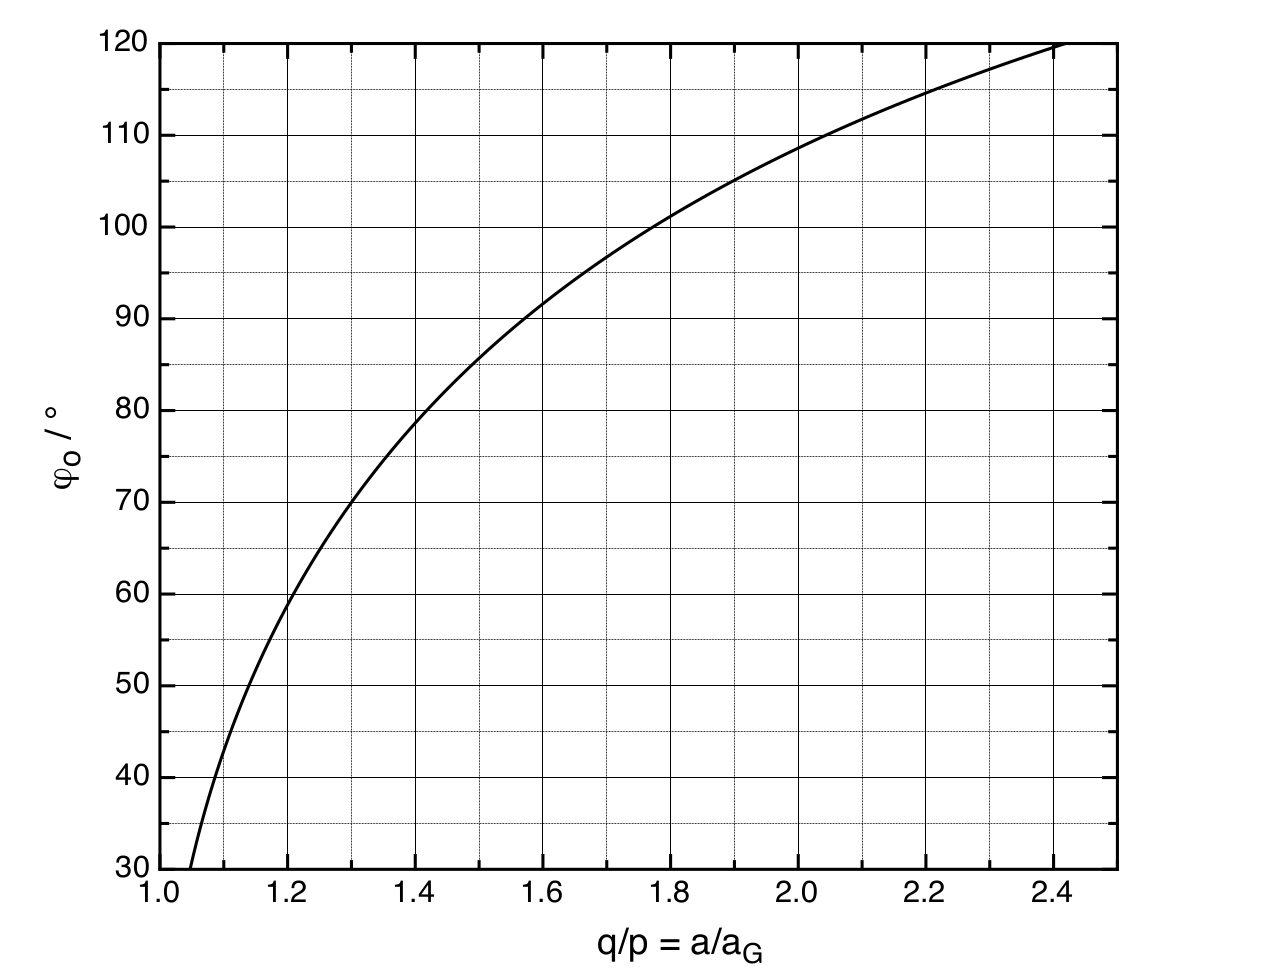
\includegraphics[width=.75\textwidth]{images/qp-plot.png}
    \caption{%
        Ruhelage des invertierten Pendels als Funktion der Ruhelage $a$ (Quelle: Versuchsanleitung)
    }
    \label{fig:qp}
\end{figure}
